%%%%%%%%%%%%%%%%%%%%%%%%%%%%%%%%%%%%%%%%%%%%%%%%%%%%%%%%%%%%%%%%%%%%%%%%
%                                                                      %
%     File: Thesis_Background.tex                                      %
%     Tex Master: Thesis.tex                                           %
%                                                                      %
%     Author: Andre C. Marta                                           %
%     Last modified :  2 Jul 2015                                      %
%                                                                      %
%%%%%%%%%%%%%%%%%%%%%%%%%%%%%%%%%%%%%%%%%%%%%%%%%%%%%%%%%%%%%%%%%%%%%%%%

\chapter{Background}
\label{chapter:background}

%\bigskip
%\textcolor{red}{\Large \textbf{Usar estilo diferente de referiencia aqui? Com ou sem o nome do autor?}}
%\bigskip

During the course of this work, several topics were studied in order to achieve a working and reliable system capable of producing useful data. The main part of the implementation was tied with the system architecture and signal processing to ensure no data was lost and informative measures were retrieved from the data.

As the test phase occurred in the cardiology department of \ac{hsm}, a significant part of the work was dedicated to create support for the chosen sensors and processing the data into variables known no medical teams e.g. extracting \ac{mets} \cite{crouter_METS} from accelerometry signal.

%\bigskip
%\textcolor{red}{\Large \textbf{descrever os outros metodos apresentados em vez de os referir so}}
%\bigskip
%
%\bigskip
%\textcolor{red}{\Large \textbf{nao comparar, apresentar so}}
%\bigskip

%%%%%%%%%%%%%%%%%%%%%%%%%%%%%%%%%%%%%%%%%%%%%%%%%%%%%%%%%%%%%%%%%%%%%%%%
\section{Remote Monitoring}

Collecting data from patients using very diverse systems and architectures is an evermore common and feasible practice. In \citet{b_lista} some of the most common approaches for the design and architecture of this type of systems are presented. Technology now offers a variety of technologies that can be put to use, every one of them with their own set of advantages and setbacks, most of them related with cost, coverage and ease of implementation. From the various approaches, the most commonly used and versatile is utilizing \ac{gsm} connectivity between remote sensors and a central server, this is a popular choice as it provides coverage in almost every place and is easily accessible using ubiquitous "smart" devices. \citet{b_lista} also mentions some of the general requirements of this type of systems and the main challenges still present when developing such a system. The currently proposed system covers most of the mentioned requirements, like data reliability and "comprehensive health monitoring" and solves some of the main challenges pointed like scalability, versatility and the delivery of processed and useful information to the medical teams in an easy to use interface and format.

\citet{b_lista2} presents a very complete overview of the wearable-based health monitoring systems, presenting several examples of systems and situations where this kind of setups can be useful. The main technological leaps that made the implementation of these apparatus are also presented, with miniaturization of computation and the cost-reduction of smart electronic devices playing a major part. Also \citet{wearables} talks about the main advantages and capabilities smart-wearables, with particular highlight to smartwaches. They have a seamless integration into one's life, being comfortable and as they are in almost constant contact with the wearer they can pervasively collect data without any disturbance of the subject's normal life.

There are, in the literature, some examples of systems that implement pervasive monitoring, for example the ones proposed by \citet{b_sistema_parecido} and \citet{b_sistema_parecido2a}. Most of these systems use wireless technology to perform data transmissions from a custom hardware device to a central storage. However, very few of this systems tackle practical implementation problems like scalability, integration of new sensors and even user interfaces for medical teams.

In \citet{b_sistema_parecido2} and \citet{b_sistema_parecido3} a pervasive data acquisition system is utilized with the intent of monitoring post-operative surgical patient. This system is detailed by \citet{b_sistema_parecido2a}. The architecture implemented is quite similar to the one utilized in the currently proposed system. Custom hardware (nodes) was designed to acquire bio-signals and a \ac{pda} is utilized to relay information between the \ac{bsn} and a central server. It is also mentioned the possible use of various methods for energy consumption optimization, like different \ac{rf} communication methods and energy scavenging.

Other studies propose systems that are quite comparable to the presented here. \Citet{b_sistema_parecido} proposes a system with many similarities, it is versatile and includes many different sensors with the same architecture. The main point of distinction is the medical personnel oriented interface that makes the system more configurable as the medical teams can choose which sensors to use with each patient.

\section{Privacy}

When dealing with patients' data, privacy is always a must-have concern. In \citet{b_data_pervasive} and \citet{b_data} remarks are made concerning what procedures and practices must be in place to protect data's integrity and security. The main aspects to consider are data transmission encryption, access control, data anonymity and permission control. This aspects were a major concern when developing the proposed system as described in \cref{chapter:privacy}.


\section{ECG}

\ac{ecg} is the recorded electrical activity of the heart muscle. This recording can be made with electrodes in a variety of standardized positions within the body as depicted in \cref{figure:ecg_leads}. Each electrode location will reflect in different signal morphologies that may contain different information and even contain clues to different pathologies. The most commonly viewed morphology is depicted in \cref{figure:ecg}.

\begin{figure}[!h]
	\centering
	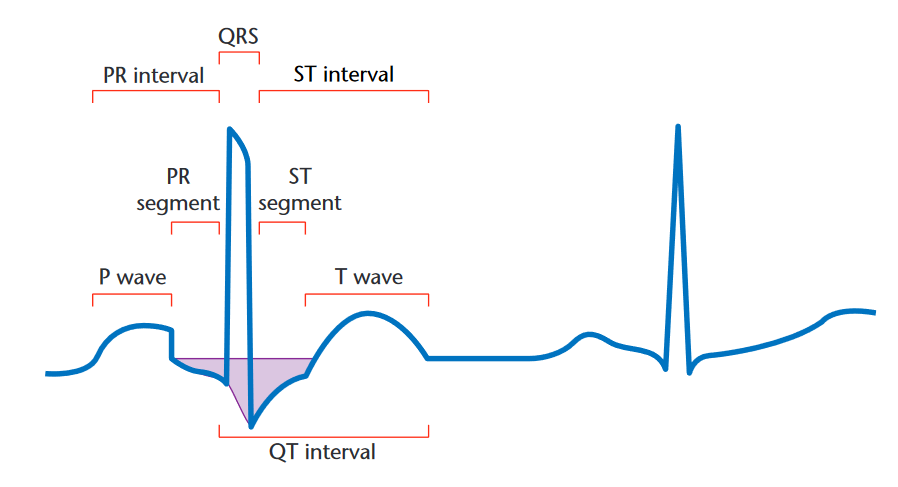
\includegraphics[width=0.75\textwidth]{ecg.png}
	\caption{\citet{b_ecg} "ECG morphology recorded 
		in a lead facing the left ventricular free
		wall showing the different waves and
		intervals. Shading, atrial repolarization
		wave."}
	\label{figure:ecg}
\end{figure}

\begin{figure}[!h]
	\centering
	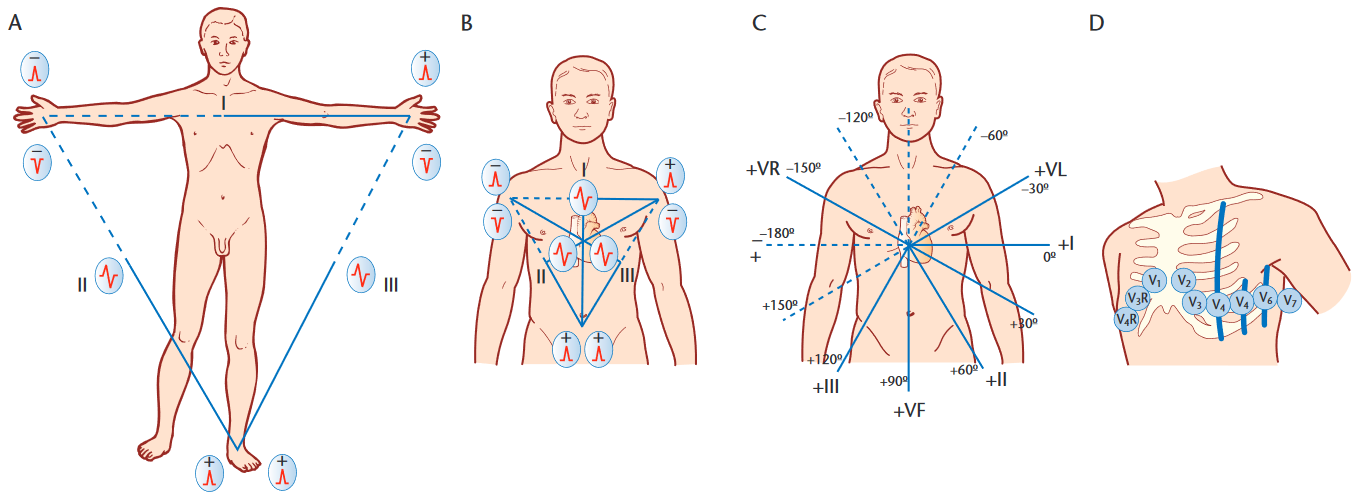
\includegraphics[width=0.90\textwidth]{ecg_leads.png}
	\caption{\citet{b_ecg} 
		"(A) Einthoven’s triangle. (B) Einthoven’s triangle superimposed on a human thorax. Note the positive (continuous line) and
		negative (dotted line) part of each lead. (C) Bailey’s hexaxial system. (D) Sites where positive poles of the six precordial leads are located."}
	\label{figure:ecg_leads}
\end{figure}

The test conditions of the system required the ECG signal to be processed in order to estimate the \ac{hr}. As described in \cref{chapter:Data Processing} this processing had to be made in two different situations, in real-time with limited computational resources and off-line without any computational restrictions and with maximum precision.

For the first situation the method proposed by \citet{segmenter} served as a base to build the used algorithm. Although the publication having several years, the method it proposes fulfills all the requirements the test conditions required. Being based on amplitude thresholding it runs in O(N) \cite{big_o} with very few calculations needed. In the literature it is possible to find similar algorithms to the one proposed, as in \citet{b_segmenter, b_segmenter_2, b_segmenter_3} with several more summarized in \citet{b_segmenter_revisiting}. Although these algorithms may perform slightly better, they still require much more computations over the entire length of the signal window, making them less fitted for the intended application.
%As the intended value to calculate was an approximation of the \ac{hr} over each 10s window, instantaneous \ac{hr} was not relevant and some error was admissible, allowing for the choice of the simplest algorithm.

\citet{b_segmenter} summarizes the most popular algorithms to process the \ac{qrs} and tries to determine which is the best one to process finger-based ECG, proposing a novel algorithm that is put against all others it mentions. The proposed algorithm is a real-time and very simple set of rules based on amplitude thresholding, similar to the one utilized in the present work.

In the algorithm proposed by \citet{b_segmenter_2}, several analog and digital filtering stages were implemented including bandpass and notch filters. The detection itself is made using and a convolution operation with a template QRS complex. Again, this approach presented a computational overhead t large to be feasible.

For the off-line \ac{hr} calculation, where precision was a requisite, and there were no limitations on calculation time and resources, the algorithm proposed by \citet{engzee} was the one chosen. This is a well established algorithm and although many more were proposed to do the same thing  e.g. the one by \citet{b_segmenter_revisiting}, this one remains a good choice for processing ECG signal as it was one of best rated algorithms in the comparison made by \citet{b_segmenter_engzee_comparison}.

In the present work, the \ac{ecg} sensor used was BITalino. It is a very customizable sensor platform with high quality \ac{ecg} signal as demonstrated by \citet{bitalinobatista2017experimental} and \citet{bitalinoguerreiro2013bitalino}. It is very convenient as it is a commercial product already including \ac{bt} communication.

There are many possible variations in ECG acquisition setups regarding the number of electrodes (leads) and the type of these electrodes. According with \citet{b_ecg_sensor}, there are four main types of electrodes: dry, gelled, insulated and non-contact. This aspect influences the quality of the signal, resistance to noise introduction and motion artifacts, but most of all the choice of electrodes has major design implications. Although gelled electrodes ensure the best power transfer to the sensor, they tend to be glued to the skin with some kind of adhesive. Although this is suitable for short term acquisitions, it can become a source of discomfort for long-term acquisitions and is not suitable for wearable inclusion. Regarding the dry and insulated electrodes, they are usually not adherent to the skin, making them suitable for long-term acquisitions or where ease in placing and removing the electrodes is desired. Finally the non-contact electrodes provide the most versatile range of applications and can even be placed over cloth.

In \citet{b_ecg_sensor2} an ECG sensor embedded in a t-shirt with insulated electrodes is presented, illustrating the easy integration of this sensors in the daily life of the person being monitored. This may present a major advantage regarding the adoption of systems based on this type of sensor.

Another approach is to embedd dry electrodes in a chest band. This is a popular method and was utilized by \citet{b_ecg_sensor3} in a very similar manner as in the present work. Dry electrodes are placed in a chest band with BT connectivity, sending data to a central monitor.



\FloatBarrier
\section{PPG}

\ac{ppg} acquisition is a way of estimating the \ac{bvp}, that can be used, among other, to determine the HR and, in certain conditions, the blood oxygen saturation as explained by \citet{b_ppg}. For oximetry, two \ac{led} of different wavelength are necessary, whereas for HR determination a single \ac{led} is enough.

Traditionally \ac{ppg} devices were placed in the fingers or ear lobes, however, in recent years, with the advent of wearables and smartwaches, there are many devices with wrist-worn \ac{ppg} sensors and other locations as presented by \citet{b_ppg_revisao}. Although many locations for the sensors have been proposed, wrist-worn sensors are the ones that present less inconveniences and are less prone to disturb daily life activities, as it is desired for pervasive monitoring.

There are authors that have built and designed their own custom hardware with many variations to perform PPG measurement. As an example, \citet{b_ppg_sensor} describes a wrist band designed to collect several bio-signals, including PPG used for HR determination. In addition, many commercially available products nowadays, include this type of sensor to appeal to customers who want to monitor themselves during daily life or even specifically during sports activities. This devices are evermore common and, some of them, have a good HR estimation capability as described by \citet{b_ppg_revisao2}.


Despite great potential, wearables have some drawbacks that greatly affect their usability. 
Smart- waches, in particular, position the PPG sensor in the distal portion of the posterior forearm. According with \citet{bvplee2016effective}, this is a location where PPG signal is faint due to reduced concentration of blood flow. Another major problem is signal corruption by motion artifacts as these devices tend to be heavy enough to have their own dynamics i.e. they move independently from the forearm by inertia. In addition, it is not comfortable to have the device too tight to the skin, and excessive pressure reduces superficial blood flow, thus further reducing \ac{snr}. In fact smartwaches and wearable sensors have been studied many times, for example by \citet{wearables} or \citet{sensor} and even its applicability as a source of clinical information has been proposed by some authors like \citet{compare, relogioarritmia} and \citet{doenca2}. However, the accuracy of this type of devices has been questioned and error margins for HR estimates produced by smartwaches were proven considerable for some devices by authors like \citet{compare, outroswearables} or \citet{compare2}.


As presented by \citet{b_ppg_revisao}, the use of green LEDs in PPG sensors is an evermore popular tendency and is the case of the sensor utilized in the currently proposed system. However this wavelength is not the ideal for this task as it is absorbed by tissues in a greater proportion than other wavelengths, making it capable of measuring only superficial blood flow. Despite the grater absorption of green light, this wavelength is, in fact, one of the the most absorbed by oxyhaemoglobin and deoxyhaemoglobin when compared to the usual red and infrared wavelengths, so it is possible to obtain better SNR although at shorter depths.

\begin{figure}[!h]
	\centering
	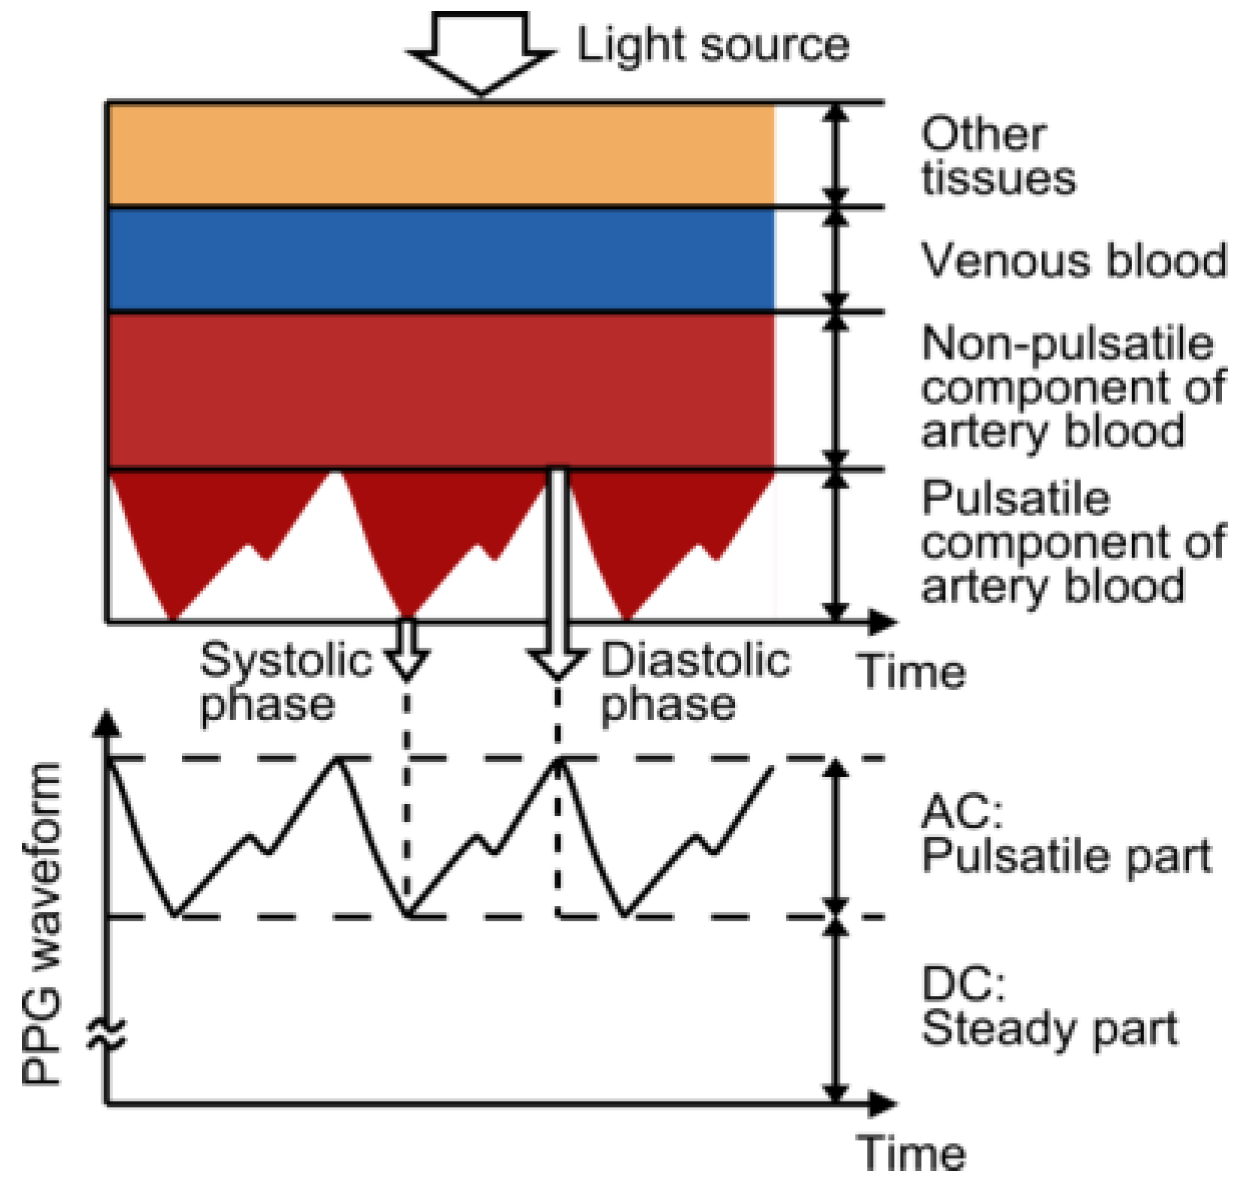
\includegraphics[width=0.6\textwidth]{ppg.png}
	\caption{\citet{b_ppg_revisao} 
		"Variation in light attenuation by tissue."}
	\label{figure:ppg}
\end{figure}

\begin{figure}[!h]
	\centering
	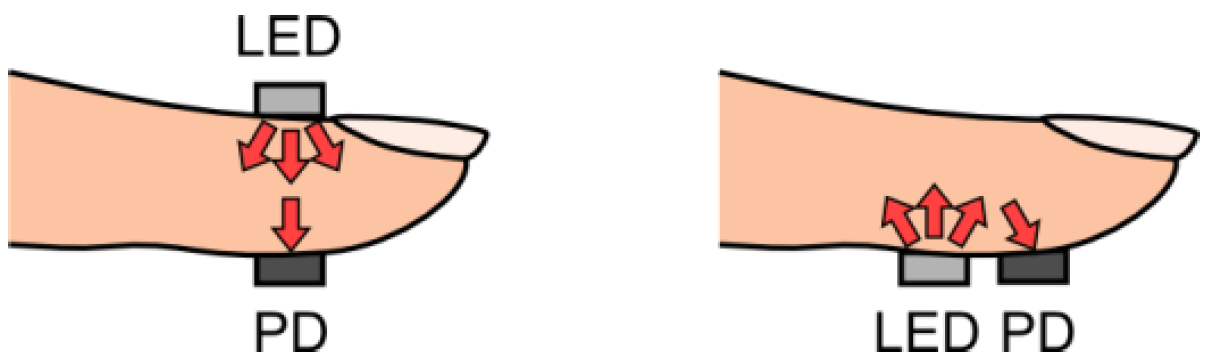
\includegraphics[width=0.8\textwidth]{ppg2.png}
	\caption{\citet{b_ppg_revisao} 
		" Light-emitting diode (LED) and photodetector (PD) placement for transmission- and reflectance-mode photoplethysmography (PPG)."}
	\label{figure:ppg2}
\end{figure}

As depicted in \cref{figure:ppg2}, there are two main types of PPG sensor, detecting transmitted and reflected light. Each of these types of sensors has their own set of positive and negative aspects. Transmission sensors have placing limitations, as not every part of the body is suitable for light to be transmitted in a practical way. This limitation makes reflection sensors the appropriate ones for wearable devices. However, reflection sensors are more sensitive to noise, as motion artifacts, mainly, can ruin the signal. To deal with this difficulty several algorithmic approaches have been developed.

As motion artifacts are one of the most prominent noise sources, most algorithm are designed to address it specifically, and not random noise like in other applications.

The simplest approach to PPG signal processing is the detection of signal features like the systolic peak, onset or others. This type of approaches were compared by \citet{bvponsetblazek2010multi} and evaluated on the performance in detecting onset, systolic peak or dicrotic notch of the PPG signal. Although this is, theoretically, enough to determine the HR from the PPG signal, in practice, this methods are very prone to error when noise is present in the signal. As this family of methods highly depends on the morphology of the signal, with the introduction of noise and motion artifacts the detection error increases very fast.

One of the most common approaches to motion artifact removal is adaptive filtering, as described by \citet{b_ppg_revisao}. There are many techniques based on this principle, that most frequently sets on the assumption of interference between the measured PPG signal and accelerations, usually measured with an accelerometer positioned in the same device as the PPG sensor. This interference can be modeled in many different ways, but most authors describe it as being a linear combination, many times simply additive i.e. the captured PPG signal is a linear combination of the true PPG signal and  a linear transformation of acceleration. This was the model used by \citet{laguerrewood2006active} to decorrelate ACC signal from the acquired PPG signal. In addition, the authors included one step of representing the signal with Laguerre coefficients before applying the adaptive filtering, this allows for a reduction of dimensionality, thus, decreasing the computational burden of the algorithm, while increasing its performance.

A different approach used by \citet{zhang2015joss} and \citet{zhang2015troika} is to look to the spectrum of the signal and reconstruct it using carefully chosen \ac{fft} segments. This works well even when there is in-band ACC noise i.e. when the spectral power of the motion artifacts is non-neglectable in the same regions as the relevant bandwidth PPG signal components.


%\bigskip
%\textcolor{red}{\Large \textbf{Reescrever}}
%\bigskip
%
%Due to poor quality PPG signal acquired, several algorithms were used in an attempt to get better HR estimates.
%Algorithms used included adaptive filtering with and without Laguerre expansion \cite{adagibbs2005active,laguerrewood2006active}, signal separation by sparse signal reconstruction \cite{zhang2015joss,zhang2015troika} and onset detection \cite{bvponsetblazek2010multi}. A total of 8 algorithms were used to process the PPG and accelerometry data coming from S3 to produce estimates of HR. However, the results obtained using all this algorithms performed equally bad, or even worse, than Gear's algorithm and for this reason, they were not mentioned previously. This clearly indicates that elevated error in Gear's HR estimations is probably related with a low quality signal and not with a poorly performing algorithm.
%
%\bigskip
%\textcolor{red}{\Large \textbf{------------------}}
%\bigskip

%\subsection{ACC  Processing}
%
%\bigskip
%\textcolor{red}{\Large \textbf{ACC}}
%\bigskip

\section{Physical activity}

Physical activity estimation can be useful in a variety of scenarios, from sports performance tracking, to patient recovery monitoring. Although a method to take this measurement may, intuitively, not be obvious, there are a few different ways of doing so. The main methods used are questionnaires, GPS monitoring and the extraction of indicators from \ac{acc} signals. All of them have downsides, and may not be suitable to cover all situations. Intuitively it is easy to understand that self-reported physical activity level is very prone to error. On the other hand GPS quantification is only suitable for activities implying great dislocations, as the GPS is not suitable for exercises in a gym environment for example. Finally accelerometry has a considerable disadvantage as the location of the sensors on the body conditions the type of activities it can successfully record, and most type having a full body monitoring is not practical nor possible.


\ac{acc} sensors are used to measure the acceleration they are subjected to, and when incorporated into a wearable device they can be used to detect movements and even estimate the physical activity level of the wearer as it was made by \citet{b_acc}. In this study, the purpose was to quantify the physical activity for different age groups. For this, subjects were asked to wear the measuring devices for 7 days and quantification was made using \ac{mets}. This is a popular way to quantify physical activity and it can be calculated from \ac{acc} data as defined by \citet{crouter_METS}.

Another approach to the physical activity analysis is trying to identify the activity being performed, in spite of trying to quantify its intensity. Many authors proposed methods for doing this type of activity recognition. \citet{b_acc2} presented a review of current methods for accomplishing this task. Methods are usually divided into similar stages with the collection of data, that is preprocessed, and then fed into some type of classifier producing the identification. Alongside algorithms to process ACC data, also video capture is a popular approach, although, only suitable for studying subjects in controlled environments, as opposed to daily life monitoring. 

\section{Data compression}

Regarding data compression for storing and relaying, some requirements were established, mainly related with performance and complexity of algorithms. Concerning the computational burden, the algorithms used had to be as simple and efficient as possible to reduce resource expenditure whereas for the algorithms themselves, they had to be lossless and it should be possible to compress segments of the signal, instead of having an algorithm compress the whole data.

There are many types of data compression algorithms, and the majority exploits some statistical property to find a smaller representation of the data. Although some algorithms are built to deal with a particular format of data, as the ones in \citet{b_ecg_compression} and \citet{b_ecg_compression_2} for example. However to maintain the versatility of the proposed system, the chosen algorithms to perform this task must be completely general on the signals to be compressed. For this reason, all data is seen as text strings, and like so, when compressing them as text, no data is lost and statistical properties become clearer when compared with numerical ones i.e. to represent numbers as strings only 12 symbols are needed (0-9, "-" and ".") eliminating the need to cover the range of each signal's value. At the same time, memory is limited and data size is relatively small, further limiting algorithm choice.

In \citet{b_textcompression} many algorithms are presented to perform data compression. However when taking into account the required utmost simplicity, Huffman static codding and time differencing were the chosen alternative.

%\bigskip
%\textcolor{red}{\Large \textbf{activity recognitin}}
%\bigskip

%%%%%%%%%%%%%%%%%%%%%%%%%%%%%%%%%%%%%%%%%%%%%%%%%%%%%%%%%%%%%%%%%%%%%%%%
%\section{Signal Processing}
%\label{section:theory1}
%
%\subsection{ECG Processing}
%
%
%\begin{figure}[!h]
%	\centering
%	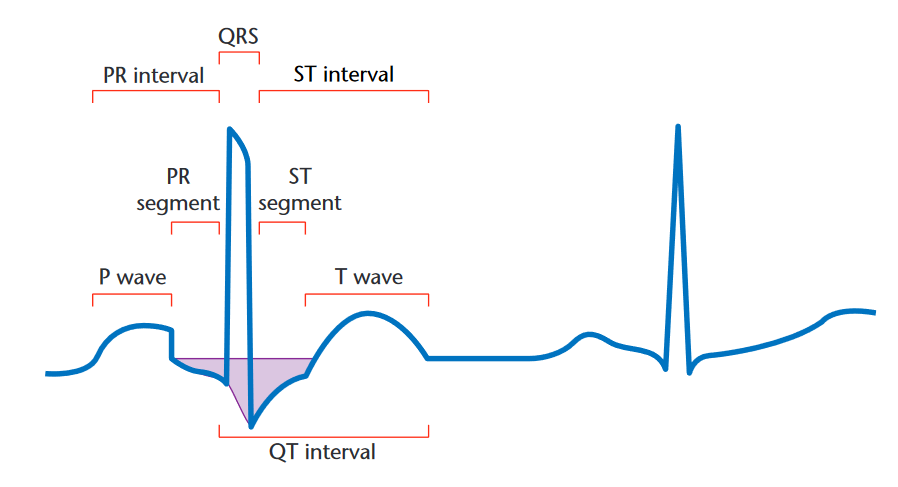
\includegraphics[width=0.85\textwidth]{ecg.png}
%	\caption{\citet{b_ecg} "ECG morphology recorded 
%		in a lead facing the left ventricular free
%		wall showing the different waves and
%		intervals. Shading, atrial repolarization
%		wave."}
%	\label{figure:ecg}
%\end{figure}
%
%\begin{figure}[!h]
%	\centering
%	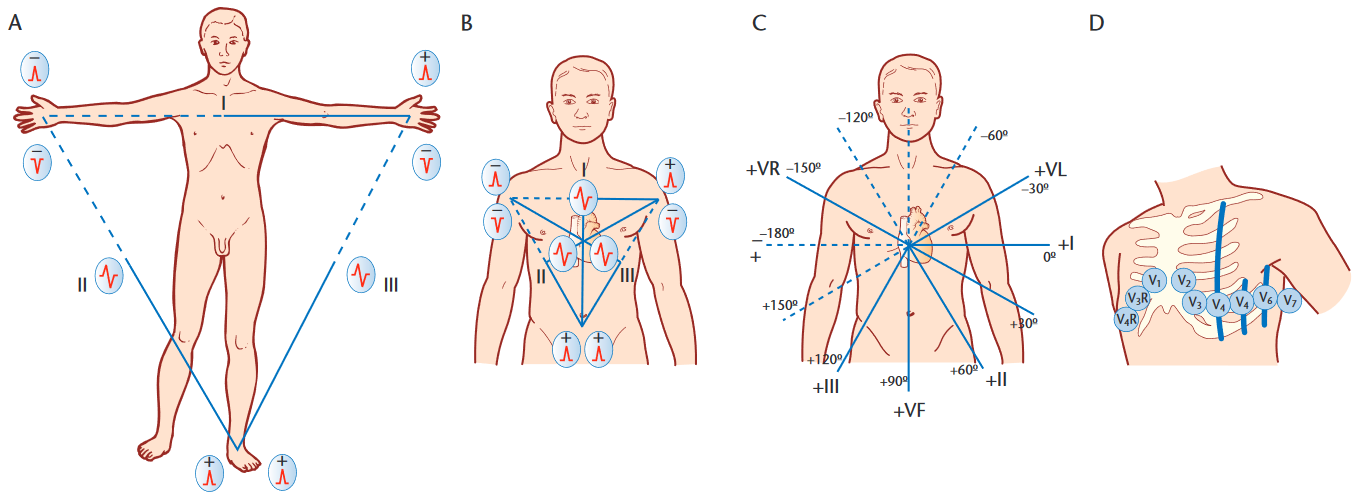
\includegraphics[width=0.90\textwidth]{ecg_leads.png}
%	\caption{\citet{b_ecg} 
%		"(A) Einthoven’s triangle. (B) Einthoven’s triangle superimposed on a human thorax. Note the positive (continuous line) and
%		negative (dotted line) part of each lead. (C) Bailey’s hexaxial system. (D) Sites where positive poles of the six precordial le
%		ads are located."}
%	\label{figure:ecg_leads}
%\end{figure}
%
%ECG is the recorded electrical activity of the heart muscle. This recording can be made with electrodes in a variety of standardized positions within the body as depicted in \cref{figure:ecg_leads}. Each electrode location will reflect in different signal morphologies that may contain different information. The mos commonly viewed morphology is depicted in \cref{figure:ecg}.
%
%The test conditions of the system required the ECG signal to be processed in order to estimate the \ac{hr}. As described in \cref{chapter:Data Processing} this processing had to be made in two different situations, in real-time with limited computational resources and off-line with no restrictions and with maximum precision.
%
%For the first situation the method proposed by \citet{segmenter} served as a base to build the used algorithm. Although the publication having several years, the method it proposes fulfills all the requirements the test conditions required. Being based on amplitude thresholding it runs in O(N) with very few calculations needed \cite{big_o}. In the literature it is possible to find similar algorithms to the one proposed, as in \citet{b_segmenter, b_segmenter_2, b_segmenter_3} with several more summarized in \citet{b_segmenter_revisiting}. Although these algorithms may perform slightly better, they still require much more computations over the entire length of the signal window.
%%As the intended value to calculate was an approximation of the \ac{hr} over each 10s window, instantaneous \ac{hr} was not relevant and some error was admissible, allowing for the choice of the simplest algorithm.
%
%\citet{b_segmenter} summarizes the most popular algorithms to process the \ac{qrs} and tries to determine what is the best to process finger-based ECG, and also proposing another algorithm. The proposed algorithm is a real-time and very simple set of rules based on amplitude thresholding, similar to the one utilized in the present work.
%
%In the algorithm proposed by \citet{b_segmenter_2}, several analog and digital filtering stages were implemented including bandpass and notch filters. The detection itself is made using and a convolution operation with a template QRS complex.
%
%For the off-line \ac{hr} calculation, where precision was a requisite, and there were no limitations os calculation time and resources, the algorithm proposed in \citet{engzee} was the one chosen. This is a well established algorithm and although many more were proposed to do the same thing \citet{b_segmenter_revisiting}, this one remains a good choice for processing ECG signal as it was one of best rated algorithms in the comparison made by \citet{b_segmenter_engzee_comparison}.



%\subsection{PPG Processing}
%
%As presented by \citet{b_ppg_revisao}, the use of green LEDs in PPG sensors is an evermore popular tendency and is the case of the sensor utilized in the currently proposed system. However this wavelength is not the ideal for this task as it is absorbed by tissues in a greater proportion than other wavelengths, making it capable of measuring only superficial blood flow. Despite the grater absorption of green light, this wavelength is, in fact, one of the the most absorbed by oxyhaemoglobin and deoxyhaemoglobin compared to infrared light, so it is possible to obtain better SNR although at shorter depths.
%
%\begin{figure}[!h]
%	\centering
%	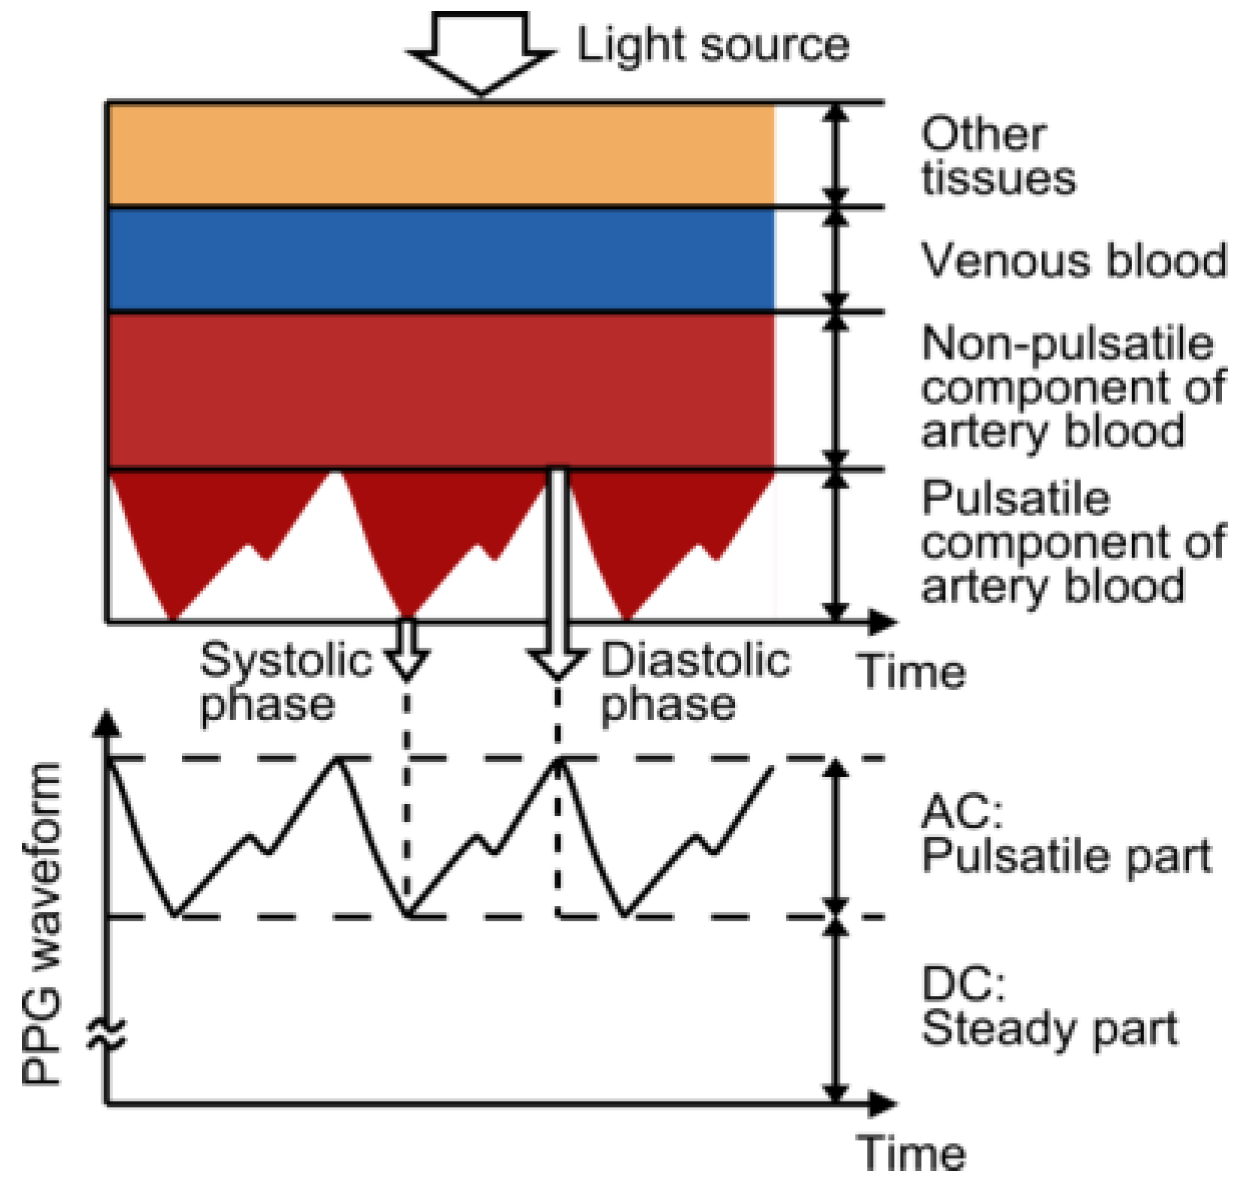
\includegraphics[width=0.90\textwidth]{ppg.png}
%	\caption{\citet{b_ppg_revisao} 
%		"Variation in light attenuation by tissue."}
%	\label{figure:ppg}
%\end{figure}
%
%\begin{figure}[!h]
%	\centering
%	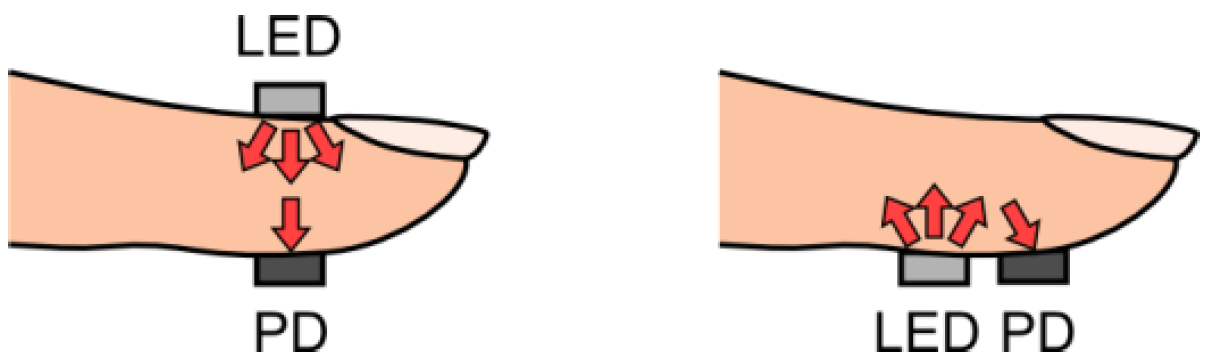
\includegraphics[width=0.90\textwidth]{ppg2.png}
%	\caption{\citet{b_ppg_revisao} 
%		" Light-emitting diode (LED) and photodetector (PD) placement for transmission- and reflectance-mode photoplethysmography (PPG)."}
%	\label{figure:ppg}
%\end{figure}
%
%\bigskip
%\textcolor{red}{\Large \textbf{Reescrever}}
%\bigskip
%
%Due to poor quality PPG signal acquired, several algorithms were used in an attempt to get better HR estimates.
%Algorithms used included adaptive filtering with and without Laguerre expansion \cite{adagibbs2005active,laguerrewood2006active}, signal separation by sparse signal reconstruction \cite{zhang2015joss,zhang2015troika} and onset detection \cite{bvponsetblazek2010multi}. A total of 8 algorithms were used to process the PPG and accelerometry data coming from S3 to produce estimates of HR. However, the results obtained using all this algorithms performed equally bad, or even worse, than Gear's algorithm and for this reason, they were not mentioned previously. This clearly indicates that elevated error in Gear's HR estimations is probably related with a low quality signal and not with a poorly performing algorithm.
%
%\bigskip
%\textcolor{red}{\Large \textbf{------------------}}
%\bigskip
%
%%\subsection{ACC  Processing}
%%
%%\bigskip
%%\textcolor{red}{\Large \textbf{ACC}}
%%\bigskip



%\begin{itemize}
%  \item Citation mode \#1 - \quad \cite{telemold}
%  \item Citation mode \#2 - \quad \citet{telemold}
%  \item Citation mode \#3 - \quad \citep{telemold}
%  \item Citation mode \#4 - \quad \citet*{telemold}
%  \item Citation mode \#5 - \quad \citep*{telemold}
%  \item Citation mode \#6 - \quad \citealt{telemold}
%  \item Citation mode \#7 - \quad \citealp{telemold}
%  \item Citation mode \#8 - \quad \citeauthor{telemold}
%  \item Citation mode \#9 - \quad \citeyear{telemold}
%  \item Citation mode \#10 - \quad \citeyearpar{telemold}
%\end{itemize}



